% For LaTeX-Box: root = stat105_F15_exam1B.tex 
%%%%%%%%%%%%%%%%%%%%%%%%%%%%%%%%%%%%%%%%%%%%%%%%%%%%%%%%%%%%%%%%%%%%%%%%%%%%%%%%
%  File Name: stat105_F15_exam1B.tex
%  Purpose:
%
%  Creation Date: 24-09-2015
%  Last Modified: Mon Oct  2 13:57:00 2017
%  Created By:
%%%%%%%%%%%%%%%%%%%%%%%%%%%%%%%%%%%%%%%%%%%%%%%%%%%%%%%%%%%%%%%%%%%%%%%%%%%%%%%%
\documentclass[addpoints]{examsetup}\usepackage[]{graphicx}\usepackage[]{color}
%% maxwidth is the original width if it is less than linewidth
%% otherwise use linewidth (to make sure the graphics do not exceed the margin)
\makeatletter
\def\maxwidth{ %
  \ifdim\Gin@nat@width>\linewidth
    \linewidth
  \else
    \Gin@nat@width
  \fi
}
\makeatother

\definecolor{fgcolor}{rgb}{0.345, 0.345, 0.345}
\newcommand{\hlnum}[1]{\textcolor[rgb]{0.686,0.059,0.569}{#1}}%
\newcommand{\hlstr}[1]{\textcolor[rgb]{0.192,0.494,0.8}{#1}}%
\newcommand{\hlcom}[1]{\textcolor[rgb]{0.678,0.584,0.686}{\textit{#1}}}%
\newcommand{\hlopt}[1]{\textcolor[rgb]{0,0,0}{#1}}%
\newcommand{\hlstd}[1]{\textcolor[rgb]{0.345,0.345,0.345}{#1}}%
\newcommand{\hlkwa}[1]{\textcolor[rgb]{0.161,0.373,0.58}{\textbf{#1}}}%
\newcommand{\hlkwb}[1]{\textcolor[rgb]{0.69,0.353,0.396}{#1}}%
\newcommand{\hlkwc}[1]{\textcolor[rgb]{0.333,0.667,0.333}{#1}}%
\newcommand{\hlkwd}[1]{\textcolor[rgb]{0.737,0.353,0.396}{\textbf{#1}}}%

\usepackage{framed}
\makeatletter
\newenvironment{kframe}{%
 \def\at@end@of@kframe{}%
 \ifinner\ifhmode%
  \def\at@end@of@kframe{\end{minipage}}%
  \begin{minipage}{\columnwidth}%
 \fi\fi%
 \def\FrameCommand##1{\hskip\@totalleftmargin \hskip-\fboxsep
 \colorbox{shadecolor}{##1}\hskip-\fboxsep
     % There is no \\@totalrightmargin, so:
     \hskip-\linewidth \hskip-\@totalleftmargin \hskip\columnwidth}%
 \MakeFramed {\advance\hsize-\width
   \@totalleftmargin\z@ \linewidth\hsize
   \@setminipage}}%
 {\par\unskip\endMakeFramed%
 \at@end@of@kframe}
\makeatother

\definecolor{shadecolor}{rgb}{.97, .97, .97}
\definecolor{messagecolor}{rgb}{0, 0, 0}
\definecolor{warningcolor}{rgb}{1, 0, 1}
\definecolor{errorcolor}{rgb}{1, 0, 0}
\newenvironment{knitrout}{}{} % an empty environment to be redefined in TeX

\usepackage{alltt}

\usepackage{etoolbox}
\usepackage{tikz,pgfplots}
\usepackage{graphicx, fancyhdr}
\usepackage{amsmath, amsfonts}
\usepackage{color}

%% For LaTeX-Box: root = stat105_exam1_info.tex 
%%%%%%%%%%%%%%%%%%%%%%%%%%%%%%%%%%%%%%%%%%%%%%%%%%%%%%%%%%%%%%%%%%%%%%%%%%%%%%%%
%  File Name: stat105_exam1_info.tex
%  Purpose:
%
%  Creation Date: 24-09-2015
%  Last Modified: Thu Sep 24 13:51:36 2015
%  Created By:
%%%%%%%%%%%%%%%%%%%%%%%%%%%%%%%%%%%%%%%%%%%%%%%%%%%%%%%%%%%%%%%%%%%%%%%%%%%%%%%%
\newcommand{\course}[1]{\ifstrempty{#1}{STAT 105}{STAT 105, Section #1}}
\newcommand{\sectionNumber}{B}
\newcommand{\examDate}{October 1, 2015}
\newcommand{\semester}{FALL 2015}
\newcommand{\examNumber}{II}

\newcommand{\examTitle}{Exam \examNumber}

\runningheader{\course{\sectionNumber}}{Exam \examNumber}{\examDate}
\runningfooter{}{}{Page \thepage of \numpages}

\newcommand{\examCoverPage}{
   \begin{coverpages}
   \centering
   {\bfseries\scshape\Huge Exam I \par}
   \vspace{1cm}
   {\bfseries\scshape\LARGE \course{\sectionNumber} \par}
   {\bfseries\scshape\LARGE \semester \par}

   \vspace{2cm}

   \fbox{\fbox{\parbox{5.5in}{\centering 

      \vspace{.25cm} 
      
      {\bfseries\Large Instructions} \\

      \vspace{.5cm} 

      \begin{itemize}
         \item  The exam is scheduled for 80 minutes, from 8:00 to 9:20 AM. At 9:20 AM the exam will end.\\
         \item  A forumula sheet is attached to the end of the exam. Feel free to tear it off.\\
         \item  You may use a calculator during this exam.\\
         \item  Answer the questions in the space provided. If you run out of room, continue on the back of the page. \\
         \item  If you have any questions about, or need clarification on the meaning of an item on this exam, please ask your instructor. No other form of external help is permitted attempting to receive help or provide help to others will be considered cheating.\\
         \item  {\bfseries Do not cheat on this exam.} Academic integrity demands an honest and fair testing environment. Cheating will not be tolerated and will result in an immediate score of 0 on the exam and an incident report will be submitted to the dean's office.\\
      \end{itemize}

   }}}

   \vspace{2cm}

   \makebox[0.6\textwidth]{Name:\enspace\hrulefill}

   \vspace{1cm}

   \makebox[0.6\textwidth]{Student ID:\enspace\hrulefill}
   \end{coverpages}

}


\newcommand{\course}[1]{\ifstrempty{#1}{STAT 105}{STAT 105, Section #1}}
\newcommand{\sectionNumber}{B}
\newcommand{\examDate}{November 5, 2015}
\newcommand{\semester}{FALL 2015}
\newcommand{\examNumber}{II}

%%%%%%%%%%%%%%%%%%%%%%%%%%%%%%%%%%%%%%%%%%%%%%%%%%%%%%%%%%%%%%%%%%%%%%%%%%%%%%%%
\IfFileExists{upquote.sty}{\usepackage{upquote}}{}
\begin{document}

%-- : R code (Code in Document)



\examCoverPage

\begin{questions}

\question[15] 

\textbf{High pressure fracking} is the process of drilling down into the earth and then injecting a high-pressure mixture called "fracking fluid" into the wellbore, the resulting pressure of which forces the release of petroleum from the sediment below.
A company specializing in the production of the fracking fluid, which is primarily water and sand, is interested in determining the how the rate of flow of the gas (in liters per second) relates to the amount of sand in the fracking fluid and the type of rock from which the petroleum is being extracted.
The have performed this process using three different mixtures of fracking fluid (high sand, medium sand, and low sand) and two types of sediment (high petroleum and low petroleum). 
They tested each combination of fracking fluid type and sediment type three times, with the results recorded in the table below:

%-- : R code (Code in Document)


\begin{table}[h]
\centering
\begin{tabular}{lrr}
 & \multicolumn{2}{c}{Sediment} \\
\cline{2-3}
Fluid & Low Petroleum & High Petroleum \\ \hline \hline
Low Sand & 4.23 & 9.87 \\
          & 4.08 & 9.23 \\
          & 3.81 & 8.86 \\
Medium Sand & 4.57 & 10.48 \\
            & 4.49 & 9.91 \\
            & 4.42 & 10.45 \\
High Sand & 3.76 & 10.1 \\
         & 3.77 & 8.93 \\
         & 3.84 & 9.37 \\
\hline
\end{tabular}
\end{table}

The engineer tasked with analyzing this data assigns the fluid to Factor A and assigns the levels to integers: Low = 1, Medium = 2, High = 3.
She also assigns the sediment to "Factor B" and the sediment types to integers: Low = 1, High = 2.

The following summaries may help in this problem:

%-- : R code (Code in Document)


% \begin{table}[h]
% \centering
% \begin{tabular}{lrrr}
%  & \multicolumn{2}{c}{Sediment} \\
% \cline{2-3}
% Fluid & Low Petroleum & High Petroleum \\ \cline{1-3} \cline{1-3}
% Low Sand & $\bar{y}_{11} = y11$ & $\bar{y}_{12} = y12$  & $\bar{y}_{1.} = y1dot$ \\
% Medium Sand & $\bar{y}_{21} = y21$ & $\bar{y}_{22} = y22$  & $\bar{y}_{2.} = y2dot$ \\
% High Sand & $\bar{y}_{31} = y31$ & $\bar{y}_{32} = y32$  & $\bar{y}_{3.} = y3dot$ \\ \cline{1-3}
% & $\bar{y}_{.1} = ydot1$ & $\bar{y}_{.2} = ydot2$  & $\bar{y}_{..} = ydotdot$ \\
% \end{tabular}
% \end{table}

\begin{table}[h]
\centering
\begin{tabular}{lrrr}
 & \multicolumn{2}{c}{Sediment} \\
\cline{2-3}
Fluid & Low Petroleum & High Petroleum \\ \cline{1-3} \cline{1-3}
Low Sand &                              & $\bar{y}_{12} = 9.32$  &  \\
Medium Sand & $\bar{y}_{21} = 4.49$ & $\bar{y}_{22} = 10.28$  & $\bar{y}_{2.} = 7.38$ \\
High Sand & $\bar{y}_{31} = 3.79$ & $\bar{y}_{32} = 9.47$  &  \\ \cline{1-3}
& $\bar{y}_{.1} = 4.11$ &   & $\bar{y}_{..} = 6.9$ \\
\end{tabular}
\end{table}


\vspace{1cm}

\begin{parts}

   \part[2] Report the value of $\bar{y}_{1.}$.
   \vspace{2cm}

   \part[2] Report the value of $\bar{y}_{3.}$.
   \vspace{2cm}

   \part[2] Report the value of $\bar{y}_{.2}$.
   \vspace{2cm}

   \newpage

   \part[5] Using the template below, create a profile plot for this data:

%-- : R plot (results in document)
\begin{knitrout}
\definecolor{shadecolor}{rgb}{0.969, 0.969, 0.969}\color{fgcolor}
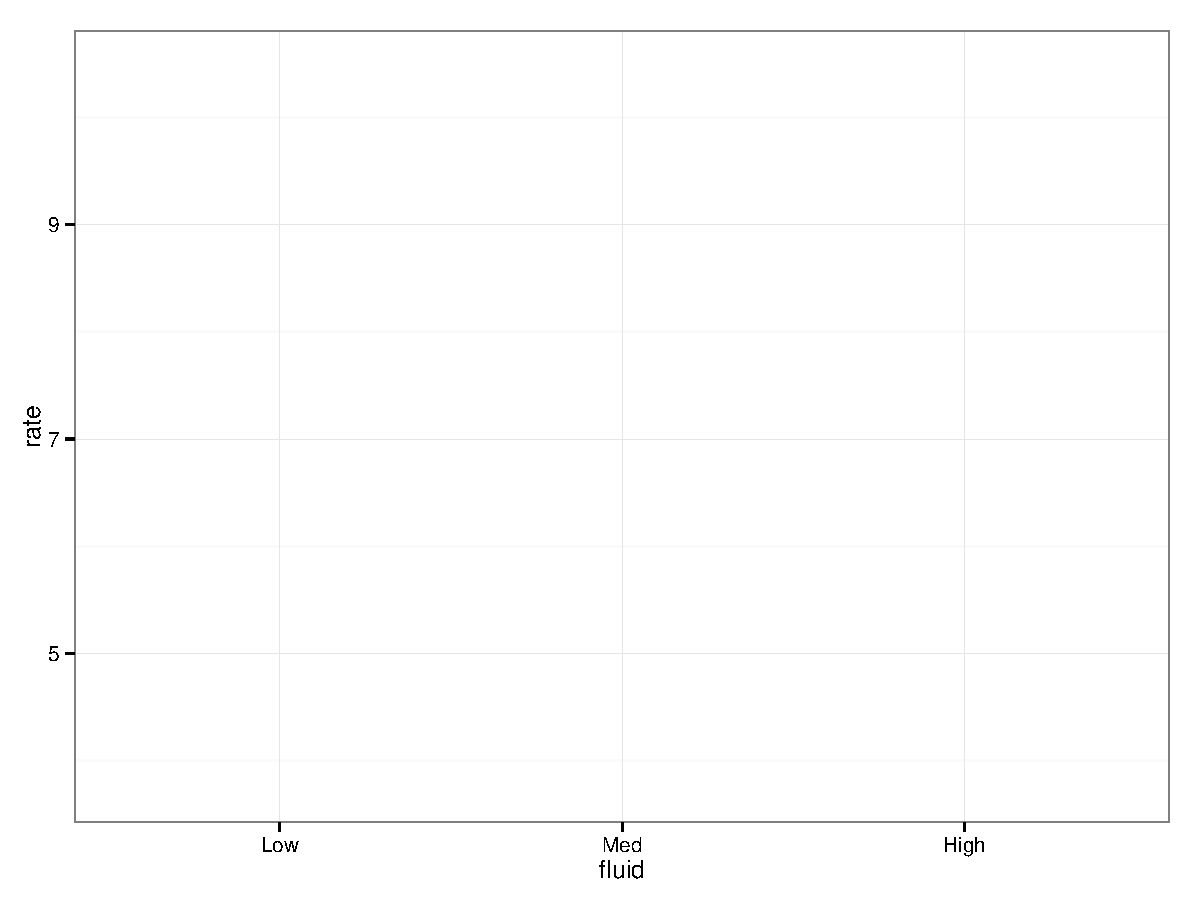
\includegraphics[width=.9\linewidth]{figure/unnamed-chunk-4-1} 

\end{knitrout}

   \part[2] Using the plot does it appear that there is an  interaction between fluid type and sediment type? Justify your answer.
   \vspace{2cm}


   \part[2] Ignoring possible interactions, find the fitted main effect of using the fluid with a low sand level, $a_1$.
   \vspace{2cm}

   \part[2] Ignoring possible interactions and fitting a factorial model without interaction effects, find the best estimate of the response when fluid is at level 1 and sediment is at level 2.
   \vspace{2cm}

\end{parts}

\newpage

\question 

Danny Ocean has a rigged pair of die (one red and one blue) that he plans to sneak into a casino game in which large payouts are given when either a roll 7 or 11 is observed and the player loses the bet for any other outcome. 
Since Mr. Ocean is knowledgable on statistics, he knows that we can consider the number of dots facing up on each die as random variables.
He calls the number of dots on the red die $X$ and the number of dots on the blue die $Y$.
The probability functions for the two are partially recorded below:

%-- : R code (Code in Document)



%  \begin{table}[h]
%     \centering
%     \begin{tabular}{cccccccc}
%        & 1 & 2 & 3 & 4 & 5 & 6 \\
%        $f_{X}(x)$ & fx(1) & fx(2) & fx(3) & fx(4) & fx(5) & fx(6) \\
%        $f_{Y}(y)$ & fy(1) & fy(2) & fy(3) & fy(4) & fy(5) & fy(6) \\
%     \end{tabular}
%  \end{table}


\begin{table}[h]
   \centering
   \begin{tabular}{cccccccc}
      & 1 & 2 & 3 & 4 & 5 & 6 \\
      $f_{X}(x)$ &               & 2/21 & 3/21 & 4/21 & 5/21 & 6/21 \\
      $f_{Y}(y)$ & 6/21 & 5/21 & 4/21 & 3/21 & 2/21 &               \\
   \end{tabular}
\end{table}

He further defines a new random variable, $W = X + Y$, the total facing up. Again, if $W = 7$ or $W = 11$ Danny wins - otherwise, he loses.

\begin{parts}

   \part[2] Find $P\left[Y = 1\right]$. 
   \vspace{1.5cm}

   \part[2] Find $f_X(1)$. 
   \vspace{1.5cm}

   \part[2] Find $P\left[Y = 6\right]$. 
   \vspace{1.5cm}

   \part[2] Find $\mathbb{E}(X)$. 
   \vspace{1.5cm}

   \part[4] Find the probability that an individual roll is a is a win for Danny. %(i.e., find $P(W = 7) + P(W = 11)$).

   \vspace{2cm}

   \part[4] Danny sneaks the die into the game but knows his ruse will be discovered if the die are rolled more than three times. Each roll is independent of the others, and he knows that the chance that he wins a single roll does not change at any point. What is the probability Danny wins two of the three bets he can make?

   \vspace{2cm}

\end{parts}

\newpage

\question

Let $X$ be a normal random variable with a mean of 10 and a varaince of 3 (i.e., $X \sim N(10,3)$) and let $Z$ be a random variable following a standard normal distribution.

\begin{parts}
 \part Find the following probabilities (note: Table B-3 may be helpful):
  \begin{subparts}
     \subpart[2] $P(Z \le 1)$

     \vspace{2cm}

     \subpart[2] $P(|Z| \le 1.5)$

     \vspace{2cm}

     \subpart[2] $P(-1 \le Z < 1.5)$

     \vspace{2cm}

     \subpart[2] $P(X > 13)$

     \vspace{2cm}

     \subpart[2] $P(|X| \le 16)$

     \vspace{2cm}

     \subpart[2] $P(|X| > 16)$

     \vspace{2cm}

  \end{subparts}

  \part[5] Find the value $a$ so that $P(- a + 10 < X < a + 10) = .6$ (approximate as needed).

\end{parts}

\newpage

\question 

Suppose that $X$ is a continuous random variable with cumulative density function (cdf).
$$
F(x) = 
\begin{cases}
   0 & x < 0 \\
   1 - e^{-3x} & x \ge 0
\end{cases}
$$

We refer to such a random variable as an exponential random variable.

\begin{parts}
\part What is the probability that $X$ takes a value greater than 3?

     \vspace{2cm}


\part What is the probability that $X$ takes a value between 1 and 3?

     \vspace{2cm}


\part Derive the probability density function, $f(x)$. 

     \vspace{2cm}


\part Find the value $f(0)$ and $f(1)$.

     \vspace{2cm}


\part Sketch the probability density function using the grid below (including the points $(0, f(0))$ and $(1, f(1))$.

\end{parts}

\newpage

\question

Consider two discrete random variables, $X$ and $Y$, where $X$ can take the value 1 or 2 with equal probability and $Y$ depends on which of the two values $X$ takes.
Suppose that the conditional distribution of $Y$ can be described using the conditional probability function $f(y|X=x)$, where
$$
f(y|X = 1) = 
\begin{cases}
   1/3 & y = 1, 2, \text{ or } 3 \\
   0 &  \text{ otherwise }
\end{cases}
$$
and
$$
f(y|X = 2) = 
\begin{cases}
   1/3 & y = 3, 4, \text{ or } 5 \\
   0 &  \text{ otherwise }
\end{cases}
$$
In this problem, $f(x,y) = P(X = x, Y = y)$ defines the joint probability function.

\begin{parts}
   \part Find $f_{Y}(3)$.
   \vspace{2cm}
   \part Find the joint probability $f(1,3)$.
   \vspace{2cm}
   \part Find the joint probability $f(2,5)$.
   \vspace{2cm}
   \part Find $f_X(2|Y = 3)$.
   \vspace{2cm}
   \part Find $P(X = 2|Y = 1)$.
   \vspace{2cm}
\end{parts}

\end{questions}

\end{document}
